\documentclass[conference]{IEEEtran}
\IEEEoverridecommandlockouts
\usepackage{cite}
\usepackage{amsmath,amssymb,amsfonts}
\usepackage{graphicx}
\usepackage{textcomp}
\usepackage{xcolor}
\usepackage{booktabs}
\usepackage{multirow}
\usepackage{array}
\usepackage{url}

\def\BibTeX{{\rm B\kern-.05em{\sc i\kern-.025em b}\kern-.08em
    T\kern-.1667em\lower.7ex\hbox{E}\kern-.125emX}}

\begin{document}

\title{Cognitive CanSat: Physics-Informed Telemetry Fusion and Multi-Tier TinyML Vision with Out-of-Distribution Guarding for Autonomous Atmospheric Sounding Probes}

\author{
\IEEEauthorblockN{Maneet Bhuyan}
\IEEEauthorblockA{\textit{Dept. of Aerospace and Avionics Engineering} \\
\textit{Cognitive CanSat Research Group}\\
Bhubaneswar, India \\
maneet.bhuyan@cansat-research.org}
\and
\IEEEauthorblockN{Soumil}
\IEEEauthorblockA{\textit{Dept. of Embedded Systems and Edge AI} \\
\textit{Cognitive CanSat Research Group}\\
Bhubaneswar, India \\
soumil@cansat-research.org}
\and
\IEEEauthorblockN{Bavesh}
\IEEEauthorblockA{\textit{Dept. of Flight Dynamics and Sensor Fusion} \\
\textit{Cognitive CanSat Research Group}\\
Bhubaneswar, India \\
bavesh@cansat-research.org}
\and
\IEEEauthorblockN{Harsh}
\IEEEauthorblockA{\textit{Dept. of Ground Control and Telemetry Systems} \\
\textit{Cognitive CanSat Research Group}\\
Bhubaneswar, India \\
harsh@cansat-research.org}
}

\maketitle

\begin{abstract}
Sub-kilogram atmospheric sounding probes (CanSats) face severe operational failures during high-velocity rocket deployment and parachute descent. Venturi dynamic-pressure depression corrupts barometric altimetry during transonic boost and pyrotechnic ejection. Parachute pendulum swing causes naive vertical-velocity division to diverge when forecasting time-to-impact (TTI). Standard convolutional neural networks (CNNs) deployed on microcontrollers with 520~KB of static random-access memory (SRAM) also misclassify out-of-distribution (OOD) laboratory or pre-flight scenes as safe landing zones. This paper presents Cognitive CanSat, a 250~g dual-tier atmospheric sounding probe that couples physics-informed telemetry fusion with a guarded three-tier Tiny Machine Learning (TinyML) vision hierarchy. Tier~1 executes 10~Hz thermodynamic and six-degree-of-freedom (6-DOF) inertial sensing over a 9600~bps 433~MHz Long Range (LoRa) link. Tier~2 runs an 8-bit integer (INT8) quantized depthwise-separable CNN (TinyLandingNet) on an ESP32-CAM core alongside a five-stage pre-inference gate (AerialVisionGuard). Across a 100-flight Monte Carlo ensemble (44,555 frames) seeded with physical bench noise floors ($\sigma_P = 0.143$~hPa, $\sigma_z = 0.423$~m), our hybrid Extended Kalman Filter (EKF) and Extra-Trees estimator reduces altitude root-mean-square error (RMSE) by 49.2\% to 0.903~m. Quantile Gradient Boosted Decision Trees (GBDT) reduce TTI countdown RMSE by 94.8\% to 2.33~s. TinyLandingNet achieves 93.04\% accuracy within a 7.15~KB flash footprint (compared against 99.68\% for MobileNetV3-Small and 99.73\% for ResNet-18), while AerialVisionGuard achieves 100\% OOD rejection on non-aerial inputs.
\end{abstract}

\begin{IEEEkeywords}
Atmospheric sounding, CanSat, Extended Kalman Filter, Out-of-Distribution (OOD) detection, Pico-satellite, Quantile Gradient Boosting, TinyML.
\end{IEEEkeywords}

\section{Introduction}
Miniature atmospheric sounding probes (CanSats) operate within a strict mass envelope of 250--350~g and a volume constraint of 66~mm diameter by 115~mm height \cite{cansat_overview}. These pico-satellite payloads must survive launch accelerations up to 8~G, pyrotechnic fairing separation shocks exceeding 5~G, and turbulent parachute descent through atmospheric boundary layers. Hardware resource constraints dictate every avionics design choice. Onboard microcontrollers such as the dual-core Xtensa LX6 (ESP32) provide only 520~KB of internal static random-access memory (SRAM) and operate under a 320~mW active power budget. Radio-frequency (RF) downlink capacity over sub-gigahertz 433~MHz Long Range (LoRa) transceivers is restricted to 9600~bps to maintain link margin across 2--5~km slant ranges \cite{lora_telemetry}. Raw video transmission requires 15,000~bytes per compressed frame and 1,450~mW of continuous RF amplifier power, which exceeds both the channel capacity and the thermal envelope of a 9~V alkaline or single-cell lithium-polymer (LiPo) power bus.

Three coupled failure modes degrade autonomous state estimation and landing hazard assessment during a CanSat mission. The first failure mode is aerodynamic dynamic-pressure corruption of the static barometer. Micro-electro-mechanical systems (MEMS) barometers such as the BMP180 and BMP280 estimate altitude above ground level (AGL) from static ambient pressure $P$ via the hypsometric equation. During a 45~m/s rocket boost or a 22~m/s delayed-chute freefall, airflow across the cylindrical chassis vents induces a Bernoulli/Venturi pressure depression:
\begin{equation}
\Delta P_q = -\frac{1}{2} c_p \rho v_z^2
\label{eq:venturi_intro}
\end{equation}
where $c_p$ is the vent pressure coefficient, $\rho$ is local dry air density, and $v_z$ is vertical velocity. Standard one-dimensional (1D) Extended Kalman Filters (EKFs) assume zero-mean Gaussian measurement noise $v_k \sim \mathcal{N}(0, R)$ \cite{kalman_baro_imu}. Aerodynamic depression violates this assumption and introduces systematic positive altitude spikes of 6--14~m at apogee separation.

The second failure mode is time-to-impact (TTI) countdown divergence under parachute pendulum dynamics. Ground recovery teams and onboard camera schedulers require an accurate countdown to touchdown. A ballistic division estimator computes $\hat{T}_{tti} = h / |v_z|$ from instantaneous altitude $h$ and vertical speed $v_z$. Under a hemispherical recovery canopy, vortex shedding excites a 1.25~Hz pendulum oscillation with pitch and roll amplitudes of $\pm 25^\circ$ to $\pm 38^\circ$. Centripetal acceleration and thermal updrafts drive instantaneous $v_z$ toward zero at the apex of each swing. The denominator $|v_z|$ approaches zero and produces countdown spikes exceeding 40~s during the final 100~m of descent.

The third failure mode is out-of-distribution (OOD) visual hallucination in edge neural networks. A nadir-facing camera paired with an onboard Convolutional Neural Network (CNN) classifies terrain into safe grass landing zones, tree canopies, urban structures, or water bodies \cite{eurosat_helber}. Softmax classifiers partition the entire input feature space into convex polytopes assigned to the training classes \cite{energy_ood_liu}. When the camera captures non-aerial scenes during laboratory bench calibration, pre-launch pad checkout, or lens-cap occlusion, a standard CNN assigns high softmax confidence ($>0.90$) to an arbitrary terrain class. A portrait of a human operator or a flat drywall surface triggers false `SAFE_LZ` advisories unless an explicit OOD pre-inference filter gates the optical pipeline.

This paper addresses all three failure modes through the following four technical contributions:
\begin{itemize}
\item We design a 250~g dual-tier electromechanical avionics architecture that isolates 10~Hz atmospheric and inertial telemetry (Tier~1, 75~g, 9600~bps LoRa) from 240~MHz optical edge inference (Tier~2, 175~g, ESP32-CAM) and streams both links into a concurrent SQLite Write-Ahead Logging (WAL) ground station database.
\item We formulate a physics-informed telemetry machine learning pipeline that blends a two-state kinematic EKF with an Extra-Trees aerodynamic bias regressor ($\alpha = 0.65$) and bounds TTI uncertainty within an 80\% prediction interval $[T_{P10}, T_{P90}]$ via Quantile Gradient Boosted Decision Trees (GBDT).
\item We develop a three-tier vision hierarchy comparing a 6,996-parameter INT8 edge model (TinyLandingNet, 7.15~KB) against CUDA-trained MobileNetV3-Small (1.52M parameters) and ResNet-18 (11.18M parameters) references, protected by a five-stage pre-inference gate (AerialVisionGuard) that combines Laplacian micro-texture variance, YCbCr chromaticity, LogSumExp free energy, and the Visible Atmospherically Resistant Index (VARI).
\item We establish a three-pillar hybrid validation benchmark that integrates physical hardware bench noise characterization ($N = 362$ packets), a 10-scenario stochastic flight test suite ($3,536$ scenario frames; $3,898$ total SQLite records), and an out-of-sample 100-flight Monte Carlo ensemble ($44,555$ frames).
\end{itemize}

The remainder of this paper is organized as follows. Section~II reviews related work in pico-satellite avionics, barometric-inertial fusion, and guarded TinyML vision. Section~III details the dual-tier hardware and dual-bridge ground station architecture. Section~IV formulates the thermodynamic equations and physics-informed telemetry models. Section~V presents the three-tier vision hierarchy and the five-stage AerialVisionGuard cascade. Section~VI describes the three-pillar experimental methodology, Section~VII analyzes the quantitative ablation results, and Section~VIII concludes with operational boundary conditions and future parafoil actuation extensions.

\section{Related Work}

\subsection{CanSat and Pico-Satellite Avionics}
Academic and competition CanSat platforms traditionally operate as passive data loggers or single-tier radio transponders \cite{cansat_overview}, \cite{cansat_design_nasa}. In \cite{lora_telemetry}, a 433~MHz LoRa link transmits barometric pressure and global positioning system (GPS) coordinates at 1--2~Hz and defers all post-processing to offline desktop scripts after payload recovery. Systems that incorporate airborne imaging typically rely on analog 5.8~GHz video transmitters or high-power Wi-Fi links to stream raw frames to a ground laptop \cite{cansat_vision_parafoil}. That approach consumes 1,200--1,850~mW of RF power, requires 15~KB of bandwidth per QVGA frame, and suffers complete frame corruption during antenna polarization blackouts when the payload tumbles faster than $90^\circ$/s. Sharing a single voltage regulator between a high-current RF power amplifier (120~mA transient spikes) and a CMOS camera sensor also induces brownout resets on single-board microcontrollers. Our dual-tier architecture eliminates raw RF video downlinks during flight and encodes the entire $3 \times 3$ spatial hazard map into a 48-byte telemetry payload.

\subsection{Barometric-Inertial Sensor Fusion}
Barometric altimeters exhibit low-frequency stability but suffer from high-frequency quantization noise and aerodynamic pressure transients, whereas MEMS accelerometers provide high-bandwidth kinematic response with quadratic double-integration drift \cite{kalman_baro_imu}. Linear and Extended Kalman Filters are widely used in sounding rockets and unmanned aerial vehicles (UAVs) to fuse barometric altitude $z_{baro}$ with vertical specific force $a_z$ \cite{uav_baro_ekf}, \cite{sounding_rocket_nav}. Standard EKF formulations model barometric error as stationary white noise with constant variance $R$. During high-speed ascent ($|v_z| > 30$~m/s) or parachute deployment shock ($>5$~G), airflow separation around the cylindrical body creates non-zero-mean pressure residuals that pull the Kalman state estimate away from true geometric altitude. Pure data-driven regressors such as Random Forests or multilayer perceptrons can learn non-linear pressure-velocity mappings \cite{breiman_rf}, but unconstrained neural or tree regressors violate kinematic continuity when extrapolating outside their training altitude envelope. Blending an analytical kinematic EKF prior with an Extra-Trees residual corrector \cite{geurts_extratrees} preserves physical state continuity while subtracting velocity-squared Venturi bias.

\subsection{Edge TinyML and OOD Detection in Aerial Robotics}
Deploying deep neural networks on microcontrollers without external pseudo-static RAM (PSRAM) requires aggressive architectural compression and 8-bit integer quantization \cite{tflite_micro_david}, \cite{cmsis_nn_lai}. Standard mobile backbones such as MobileNetV3-Small (1.52M parameters, 5.81~MB in 32-bit floating point) \cite{howard_mobilenetv3} and ResNet-18 (11.18M parameters, 42.64~MB) \cite{he_resnet} achieve $>99\%$ accuracy on the EuroSAT Sentinel-2 land-cover benchmark \cite{eurosat_helber}, but their activation tensors exceed the 520~KB SRAM limit of an ESP32 by an order of magnitude. Custom depthwise-separable architectures reduce parameter counts below $10^4$, yet compact classifiers remain highly vulnerable to OOD inputs \cite{hendrycks_msp}. In \cite{energy_ood_liu}, Helmholtz free energy computed via the LogSumExp of pre-softmax logits outperforms maximum softmax probability for OOD separation. However, logit-level energy scoring alone can still fail on low-capacity INT8 networks when presented with saturated skin tones or zero-variance indoor surfaces. Combining pre-CNN optical gates (Laplacian texture variance, YCbCr skin-tone segmentation \cite{chai_skin_ycbcr}, and spectral vegetation indices \cite{gitelson_vari}) with post-CNN free energy gating provides deterministic OOD rejection under sub-watt compute limits.

\section{Dual-Tier Hardware and Communication Architecture}

\begin{table*}[t]
\centering
\caption{Electromechanical Mass, Power, and Interface Budget Across Tier 1 and Tier 2}
\label{tab:hardware_budget}
\begin{tabular}{llccc}
\toprule
\textbf{Payload Deck} & \textbf{Subsystem Component} & \textbf{Bus / Interface} & \textbf{Active Power (mW)} & \textbf{Mass (g)} \\
\midrule
\multirow{7}{*}{Tier 1: Avionics \& Sounding Deck} 
 & ATmega328P / ESP32 Primary Flight MCU & 16 / 240~MHz Core & 85 & 7.0 \\
 & SX1278 LoRa Transceiver (Ra-02, 433~MHz) & SPI Bus (9600~bps Air) & 110 & 9.0 \\
 & MPU6050 6-Axis MEMS IMU (Accel + Gyro) & $\text{I}^2\text{C}$ (`0x68`, 400~kHz) & 12 & 3.0 \\
 & BMP180 / BMP280 Digital Barometer & $\text{I}^2\text{C}$ (`0x77`, 400~kHz) & 3 & 2.0 \\
 & DHT11 Capacitive Hygrometer \& Thermistor & 1-Wire Digital Bus & 5 & 4.0 \\
 & NEO-6M GPS Receiver + Ceramic Patch Antenna & UART (9600~baud) & 125 & 18.0 \\
 & Tier 1 Circular FR4 PCB \& Brass Standoffs & Structural Backplane & 0 & 32.0 \\
\cmidrule{2-5}
 & \textit{Tier 1 Subtotal} & \textit{10~Hz Telemetry Loop} & \textit{340} & \textit{75.0} \\
\midrule
\multirow{7}{*}{Tier 2: Optical Edge AI \& Chassis} 
 & AI-Thinker ESP32-CAM (Dual-Core Xtensa LX6) & 240~MHz Edge Compute & 260 & 22.0 \\
 & OV3660 / OV2640 Nadir CMOS Camera Module & 8-Bit DVP Parallel Ribbon & 60 & 5.0 \\
 & 3D-Printed Matte-Black PLA Cylindrical Shell & 66~mm $\times$ 115~mm Airframe & 0 & 42.0 \\
 & 3D-Printed Top \& Bottom Optical End-Caps & Nadir 14~mm Aperture Bezel & 0 & 26.0 \\
 & 9~V Alkaline / LiPo Power Pack \& Snap Harness & Isolated Dual-Rail Supply & 0 & 46.0 \\
 & Brass SMA Bulkhead, Whip Antenna \& Master Switch & RF \& Power Distribution & 0 & 16.0 \\
 & Parachute Eyebolt Linkage \& M3 Stainless Fasteners & Mechanical Load Path & 0 & 18.0 \\
\cmidrule{2-5}
 & \textit{Tier 2 Subtotal} & \textit{10--26~FPS Vision Loop} & \textit{320} & \textit{175.0} \\
\midrule
\textbf{Total Integrated Payload} & \textbf{Compliant with 350~g Competition Limit} & \textbf{Dual-Stream Architecture} & \textbf{660} & \textbf{250.0} \\
\bottomrule
\end{tabular}
\end{table*}

The Cognitive CanSat airframe is housed inside a 3D-printed matte-black polylactic acid (PLA) cylindrical shell measuring 66~mm in outer diameter and 115~mm in height. Total flight mass is 250.0~g, which provides a 28.6\% structural mass margin below the 350.0~g international CanSat competition ceiling. To prevent high-frequency digital switching noise on the camera parallel bus and transient current spikes on the LoRa RF power amplifier from corrupting analog-to-digital converter (ADC) barometric measurements, the internal payload is partitioned into two mechanically and electrically isolated decks. Table~\ref{tab:hardware_budget} details the component-level mass, interface, and power distribution across both decks.

Tier~1 (Avionics and Atmospheric Sounding Deck, 75.0~g) occupies the upper section of the cylinder beneath the recovery parachute eyebolt. The primary microcontroller polls the BMP180/BMP280 barometer (`0x77`) and MPU6050 6-axis inertial measurement unit (`0x68`) over a 400~kHz $\text{I}^2\text{C}$ bus, reads relative humidity from the DHT11 sensor via a 1-Wire digital pin, and parses National Marine Electronics Association (NMEA) sentences from the side-mounted NEO-6M GPS receiver over a 9600~baud universal asynchronous receiver-transmitter (UART) interface. Sensor acquisition executes deterministically at 10~Hz (100~ms period). Each telemetry frame is serialized into a 13-field comma-separated value (CSV) packet:
\begin{equation}
\mathcal{P}_{k} = \{T, P, z_{raw}, g_x, g_y, g_z, a_x, a_y, a_z, \phi_{lat}, \lambda_{lon}, RH, V_{bat}\}
\label{eq:csv_packet}
\end{equation}
and transmitted to the ground station via an SX1278 (Ra-02) 433~MHz LoRa module over Serial Peripheral Interface (SPI) at 9600~bps.

Tier~2 (Optical Edge AI and Power Deck, 175.0~g) occupies the lower section of the chassis and faces the nadir landing zone through a 14~mm recessed optical aperture in the bottom PLA end-cap. An AI-Thinker ESP32-CAM module (dual-core Xtensa LX6 at 240~MHz, 520~KB internal SRAM) ingests $320 \times 240$ (QVGA) frames from an OV3660 CMOS sensor over an 8-bit Digital Video Port (DVP) ribbon using direct memory access (DMA). Core~0 handles DMA frame acquisition and $64 \times 64$ bilinear downsampling. Core~1 executes the five-stage AerialVisionGuard filter, INT8 TinyLandingNet inference, and $3 \times 3$ spatial hazard gradient calculation without dynamic heap allocation (`malloc`). By allocating a fixed 92~KB static tensor arena in internal SRAM, Tier~2 completes the entire perceive-and-score cycle in 38.0~ms (16.3~ms neural inference plus DMA and pre-filtering overhead).

The ground control station runs an asynchronous Python FastAPI server connected to a dual-serial hardware bridge (`DualSerialManager`). Port~1 (`COM4` at 9600~baud) ingests the 13-field LoRa telemetry stream and validates packet framing (supporting 13-field standard strings and 14-field received signal strength indicator extensions). Port~2 (`COM5` at 460800~baud) ingests `$CAM_FRAME` base64-encoded optical diagnostic packets during bench or short-range tether tests. Both streams are committed asynchronously into a local SQLite database configured in Write-Ahead Logging (`PRAGMA journal_mode=WAL;`) mode with `NORMAL` synchronization. This database configuration supports concurrent non-blocking writes at $>500$~packets/s alongside real-time WebSocket broadcasting to the Mission Control dashboard.

\section{Physics-Informed Telemetry and Machine Learning Pipeline}

\subsection{Atmospheric Thermodynamics and 6-DOF Kinematics}
Upon receiving packet $\mathcal{P}_k$ at time step $t_k$, the ground and onboard thermodynamic engine computes four atmospheric sounding quantities relative to the calibrated launch-pad reference state $(P_0, T_0)$ captured during stationary pad tare. Geometric barometric altitude $z_{baro,k}$ is obtained from the hypsometric equation:
\begin{equation}
z_{baro,k} = \frac{T_0}{L} \left[ 1 - \left( \frac{P_k}{P_0} \right)^{\frac{R_s L}{g_0}} \right]
\label{eq:hypsometric}
\end{equation}
where $L = 0.0065$~K/m is the standard tropospheric lapse rate, $R_s = 287.05$~J/(kg$\cdot$K) is the specific gas constant for dry air, and $g_0 = 9.80665$~m/s$^2$. Dew point temperature $T_{dew,k}$ ($^\circ$C) is derived from ambient temperature $T_k$ ($^\circ$C) and relative humidity $RH_k$ (\%) via the Magnus-Tetens approximation with constants $a = 17.27$ and $b = 237.7^\circ$C:
\begin{equation}
\gamma_k = \frac{a T_k}{b + T_k} + \ln\left(\frac{RH_k}{100}\right), \quad T_{dew,k} = \frac{b \gamma_k}{a - \gamma_k}
\label{eq:magnus_tetens}
\end{equation}
Local dry air density $\rho_k$ (kg/m$^3$) and the numerical Environmental Lapse Rate ($ELR_k$, in $^\circ$C/100~m) across a vertical window $\Delta z_k = z_k - z_{k-w}$ are computed as:
\begin{equation}
\rho_k = \frac{100 P_k}{R_s (T_k + 273.15)}, \quad ELR_k = -\frac{T_k - T_{k-w}}{z_k - z_{k-w}} \times 100
\label{eq:density_elr}
\end{equation}
A negative $ELR_k < -0.5^\circ$C/100~m flags a tropospheric thermal inversion layer.

Inertial attitude (pitch $\theta_k$ and roll $\phi_k$) is fused from the 3-axis accelerometer $(a_x, a_y, a_z)$ and 3-axis gyroscope $(g_x, g_y, g_z)$ using a first-order complementary filter with coefficient $\beta = 0.96$ and sampling interval $\Delta t = t_k - t_{k-1}$:
\begin{align}
\theta_{acc,k} &= \text{atan2}\left(-a_{x,k}, \sqrt{a_{y,k}^2 + a_{z,k}^2}\right) \frac{180}{\pi} \label{eq:pitch_acc} \\
\theta_k &= \beta \left(\theta_{k-1} + g_{y,k} \Delta t\right) + (1 - \beta) \theta_{acc,k} \label{eq:complementary}
\end{align}
with an analogous update for roll angle $\phi_k$. Total specific force magnitude $|a|_k = \sqrt{a_{x,k}^2 + a_{y,k}^2 + a_{z,k}^2}$ and angular velocity magnitude $|\omega|_k = \sqrt{g_{x,k}^2 + g_{y,k}^2 + g_{z,k}^2}$ trigger deterministic hardware safety flags when $|a|_k > 4.5$~G (pyrotechnic shock), $|\omega|_k > 150^\circ$/s (aerodynamic tumble), or $|a|_k < 0.2$~G (unretarded freefall).

\subsection{Hybrid Physics-Informed Altitude Estimator}
To eliminate the Venturi dynamic-pressure depression of (\ref{eq:venturi_intro}) without sacrificing kinematic continuity, we construct a hybrid estimator that couples a two-state kinematic EKF with an Extra-Trees aerodynamic residual model. Let the kinematic state vector be $\mathbf{x}_k = [z_{ekf,k}, v_{z,k}]^T$ and the vertical net kinematic acceleration be $u_k = (a_{z,k} - 1.0) g_0$. The discrete-time state prediction and covariance propagation equations are:
\begin{align}
\hat{\mathbf{x}}_{k|k-1} &= \begin{bmatrix} 1 & \Delta t \\ 0 & 1 \end{bmatrix} \mathbf{x}_{k-1} + \begin{bmatrix} \frac{1}{2}\Delta t^2 \\ \Delta t \end{bmatrix} u_k \label{eq:ekf_pred} \\
\mathbf{P}_{k|k-1} &= \mathbf{F}_k \mathbf{P}_{k-1} \mathbf{F}_k^T + \mathbf{Q} \label{eq:ekf_cov}
\end{align}
where $\mathbf{Q} = \text{diag}(0.05, 0.25)$ models accelerometer process noise and $R = 0.742^2 = 0.55$~m$^2$ matches the measured BMP280 bench altitude variance. Standard Kalman measurement update $\mathbf{x}_k = \hat{\mathbf{x}}_{k|k-1} + \mathbf{K}_k (z_{baro,k} - \mathbf{H}\hat{\mathbf{x}}_{k|k-1})$ with $\mathbf{H} = [1, 0]$ lags behind true altitude when $z_{baro,k}$ is biased by $\Delta P_q$.

We train an ensemble of $M = 150$ extremely randomized regression trees (`ExtraTreesRegressor` \cite{geurts_extratrees}, maximum depth 16) on a 12-dimensional feature vector $\mathbf{f}_k \in \mathbb{R}^{12}$:
\begin{equation}
\mathbf{f}_k = [P_k, T_k, RH_k, z_{baro,k}, v_{z,k}, \dot{P}_k, |a|_k, a_{z,k}, |\omega|_k, \rho_k, q_{dyn,k}, \sigma_{z,5}]
\label{eq:feature_vec}
\end{equation}
where $\dot{P}_k = (P_k - P_{k-1})/\Delta t$ is the pressure rate, $q_{dyn,k} = \frac{1}{2}\rho_k v_{z,k}^2$ is estimated dynamic pressure, and $\sigma_{z,5}$ is the 5-sample rolling altitude standard deviation. The tree ensemble outputs a dynamic-pressure-compensated altitude prediction $\hat{z}_{ml,k} = \mathcal{F}_{ET}(\mathbf{f}_k)$. The final fused altitude estimate $\hat{z}_{hyb,k}$ is formed via convex combination:
\begin{equation}
\hat{z}_{hyb,k} = \alpha \hat{z}_{ml,k} + (1 - \alpha) z_{ekf,k}, \quad \alpha = 0.65
\label{eq:hybrid_blend}
\end{equation}
Cross-validation across $\alpha \in [0.0, 1.0]$ at 0.05 increments confirms that $\alpha = 0.65$ minimizes trajectory RMSE across both transonic boost and pendulum descent regimes.

\subsection{Uncertainty-Aware Time-to-Impact (TTI) Forecaster}
During parachute descent, instantaneous vertical speed $v_{z,k}$ oscillates at the canopy pendulum frequency $f_p \approx 1.25$~Hz. To prevent the singularity of $\hat{T}_{tti} = \hat{z}_{hyb,k} / |v_{z,k}|$, we formulate TTI forecasting as a supervised quantile regression problem over the feature vector $\mathbf{f}_k$ augmented with a 20-sample exponentially weighted moving average of vertical velocity $\bar{v}_{z,20}$ and drag-area ratio $q_{dyn,k}/|a|_k$. Three Gradient Boosted Decision Tree (`GradientBoostingRegressor` \cite{friedman_gbdt}) ensembles with 200 estimators and learning rate $\eta = 0.05$ are trained simultaneously. The primary point estimator minimizes squared-error loss to predict expected remaining flight time $\hat{T}_{mean,k}$. Two companion models minimize the pinball (quantile) loss function $\mathcal{L}_\tau(y, \hat{y})$ for quantile levels $\tau \in \{0.10, 0.90\}$:
\begin{equation}
\mathcal{L}_\tau(y, \hat{y}) = \max\left( \tau(y - \hat{y}), (\tau - 1)(y - \hat{y}) \right)
\label{eq:pinball_loss}
\end{equation}
This triplet produces a calibrated 80\% prediction interval $[T_{P10,k}, T_{P90,k}]$ around $\hat{T}_{mean,k}$ at every 10~Hz packet step.

\subsection{Flight Phase Classifier and Telemetry Anomaly Detector}
Autonomous camera wake-up and post-flight audit logging require real-time identification of the active mission phase. A 100-tree `RandomForestClassifier` maps $\mathbf{f}_k$ into one of six discrete flight states: `PRE_LAUNCH_PAD` ($S_0$), `BOOST_ASCENT` ($S_1$), `APOGEE_SEPARATION` ($S_2$), `PARACHUTE_DESCENT` ($S_3$), `TERMINAL_APPROACH` ($S_4$, $\hat{z}_{hyb} < 150$~m), and `TOUCHDOWN_RECOVERY` ($S_5$). A hysteresis state machine requires 3 consecutive 10~Hz predictions (300~ms) before committing a forward phase transition, which prevents chattering during shock transients. In parallel, an unsupervised 100-tree `IsolationForest` \cite{liu_isolation_forest} with contamination parameter $c = 0.03$ evaluates the average path length $E[h(\mathbf{f}_k)]$ across random feature splits to flag telemetry anomalies (RF packet dropouts, LiPo voltage sag below 3.40~V, and IMU saturation) without requiring labeled fault traces.

\section{Three-Tier Vision Hierarchy and 5-Stage OOD Guard}

\subsection{Three-Tier Neural Architecture}
To quantify the accuracy-versus-resource trade-off between sub-watt microcontroller execution and unconstrained ground-station compute, we implement and train a three-tier vision hierarchy on the EuroSAT RGB aerial dataset \cite{eurosat_helber} mapped into four operational CanSat landing classes: `SAFE_LZ` (HerbaceousVegetation, AnnualCrop, Pasture, PermanentCrop), `OBSTACLE_CANOPY` (Forest), `WATER_HAZARD` (River, SeaLake), and `CRITICAL_HAZARD` (Highway, Industrial, Residential).

Tier~1 (`TinyLandingNet`) is our custom depthwise-separable CNN tailored for the ESP32-CAM internal SRAM. The network accepts a $64 \times 64 \times 3$ RGB tensor and applies a $3 \times 3$ standard convolution ($3 \rightarrow 16$ channels, stride 2, BatchNorm, ReLU6), followed by three inverted depthwise-separable blocks ($16 \rightarrow 32 \rightarrow 64 \rightarrow 64$ channels with $3 \times 3$ depthwise and $1 \times 1$ pointwise convolutions), global average pooling, dropout ($p = 0.2$), and a $64 \rightarrow 4$ linear classifier. Total trainable parameters are 6,996 (7,320 with BatchNorm running statistics). Uncompressed 32-bit floating-point (FP32) weights occupy 27.33~KB. Post-training asymmetric INT8 quantization compresses the weights to 7.15~KB, which fits inside the ESP32 L1 instruction cache and executes in 16.3~ms on the 240~MHz Xtensa LX6 core (0.055~ms in ONNX Runtime on host CPU).

Tier~2 (`MobileNetV3-Small` \cite{howard_mobilenetv3}) is our single-board computer (Raspberry Pi~4) and lightweight ground reference. It processes $224 \times 224 \times 3$ inputs using squeeze-and-excitation inverted residual blocks with hard-swish activations. The architecture has 1,521,956 parameters (5.81~MB FP32; 1,486.3~KB INT8) and requires 17.6~ms per frame on host CPU. Tier~3 (`ResNet-18` \cite{he_resnet}) is the high-capacity ground workstation teacher network. It has 11,178,564 parameters (42.64~MB FP32; 10,916.6~KB INT8) and executes in 31.9~ms on host CPU.

\subsection{5-Stage AerialVisionGuard Pre-Inference Gate}
Every frame $I \in [0, 255]^{H \times W \times 3}$ must pass through the five-stage `AerialVisionGuard` cascade before the flight computer accepts any neural landing decision. Stage~1 is the optical exposure and sensor fault gate. It computes the global mean luminance $\mu_I = \frac{1}{HW}\sum_{x,y} Y(x,y)$ and rejects overexposed glare ($\mu_I > 248$) or ribbon-cable disconnects ($\mu_I < 12$). Stage~2 is the Laplacian micro-texture gate. Natural nadir terrain exhibits multi-scale spatial gradients from grass blades, soil granularity, or roof edges, whereas indoor laboratory walls, ceilings, and lens caps exhibit flat luminance. Stage~2 convolves the grayscale frame with the discrete $3 \times 3$ Laplacian kernel $\nabla^2$ and requires the spatial variance to exceed threshold $\tau_{lap} = 14.0$:
\begin{equation}
\text{Var}(\nabla^2 I) = \frac{1}{HW} \sum_{x,y} \left( \nabla^2 I(x,y) - \mu_{\nabla^2} \right)^2 \ge 14.0
\label{eq:laplacian_gate}
\end{equation}
Frames falling below 14.0 are rejected immediately in $<0.4$~ms without invoking the CNN.

Stage~3 is the YCbCr and RGB close-up portrait skin-tone gate, designed to reject human faces and hands during pre-flight bench testing. Pixels are transformed into the ITU-R BT.601 YCbCr color space \cite{chai_skin_ycbcr}. A pixel $(x,y)$ is flagged as human skin if it satisfies the joint chromaticity and RGB dominance constraints:
\begin{equation}
\begin{cases}
77 \le C_b(x,y) \le 127, \quad 133 \le C_r(x,y) \le 173 \\
R > 95, \ G > 40, \ B > 20, \ R > G, \ R > B, \ |R - G| > 15
\end{cases}
\label{eq:skin_gate}
\end{equation}
Let $\rho_{skin,all}$ be the global fraction of skin pixels and $\rho_{skin,ctr}$ be the fraction within the central $50\%$ crop. If $\rho_{skin,ctr} > 0.22$ and $\rho_{skin,all} > 0.14$ (with green vegetation ratio $\rho_{green} < 0.20$), Stage~3 aborts inference and returns `REJECTED_HUMAN_PORTRAIT_OOD`.

Stage~4 is the temperature-scaled LogSumExp free energy and Shannon entropy gate applied to the CNN logit vector $\mathbf{z} = [z_1, z_2, z_3, z_4]^T$. Following \cite{energy_ood_liu}, the Helmholtz free energy at temperature $T = 1.0$ and the normalized Shannon entropy $H_{norm}(\mathbf{p})$ over softmax probabilities $p_c = \exp(z_c)/\sum_j \exp(z_j)$ are defined as:
\begin{equation}
E(\mathbf{x}; T) = -T \ln \sum_{c=1}^{4} \exp\left(\frac{z_c}{T}\right), \quad H_{norm}(\mathbf{p}) = -\frac{\sum_{c=1}^{4} p_c \ln p_c}{\ln 4}
\label{eq:free_energy}
\end{equation}
In-distribution aerial scenes produce strongly negative free energy $E(\mathbf{x}) < -2.1$ and low entropy. Any frame with $H_{norm}(\mathbf{p}) > 0.82$ or maximum probability $\max_c p_c < 0.45$ is rejected as `HIGH_ENTROPY_OOD`.

Stage~5 is the Visible Atmospherically Resistant Index (VARI) spectral verification and $3 \times 3$ sector evasion synthesis. For each of the 9 spatial sub-sectors $S_{r,c}$ ($r,c \in \{0,1,2\}$), Stage~5 computes mean channel intensities $(\bar{R}_{r,c}, \bar{G}_{r,c}, \bar{B}_{r,c})$ and evaluates the atmospheric-resistant vegetation index \cite{gitelson_vari}:
\begin{equation}
\text{VARI}_{r,c} = \frac{\bar{G}_{r,c} - \bar{R}_{r,c}}{\bar{G}_{r,c} + \bar{R}_{r,c} - \bar{B}_{r,c} + \epsilon}
\label{eq:vari_index}
\end{equation}
where $\epsilon = 10^{-5}$. A `SAFE_LZ` assignment in the nadir sector $S_{1,1}$ is confirmed only if $\text{VARI}_{1,1} > 0.04$ or green chromatic excess satisfies $\bar{G}_{1,1} > 1.04 \bar{R}_{1,1}$. When $S_{1,1}$ is classified as a hazard (`RISK` $> 0.65$), the flight computer selects the highest-scoring adjacent sector $(r^*, c^*) = \arg\max_{r,c} \mathcal{S}(S_{r,c})$ and downlinks the advisory evasion heading $\psi_{evade} = \text{atan2}(c^* - 1, -(r^* - 1)) \pmod{360^\circ}$.

\section{Experimental Methodology and Three-Pillar Validation}

\begin{figure}[t]
\centering
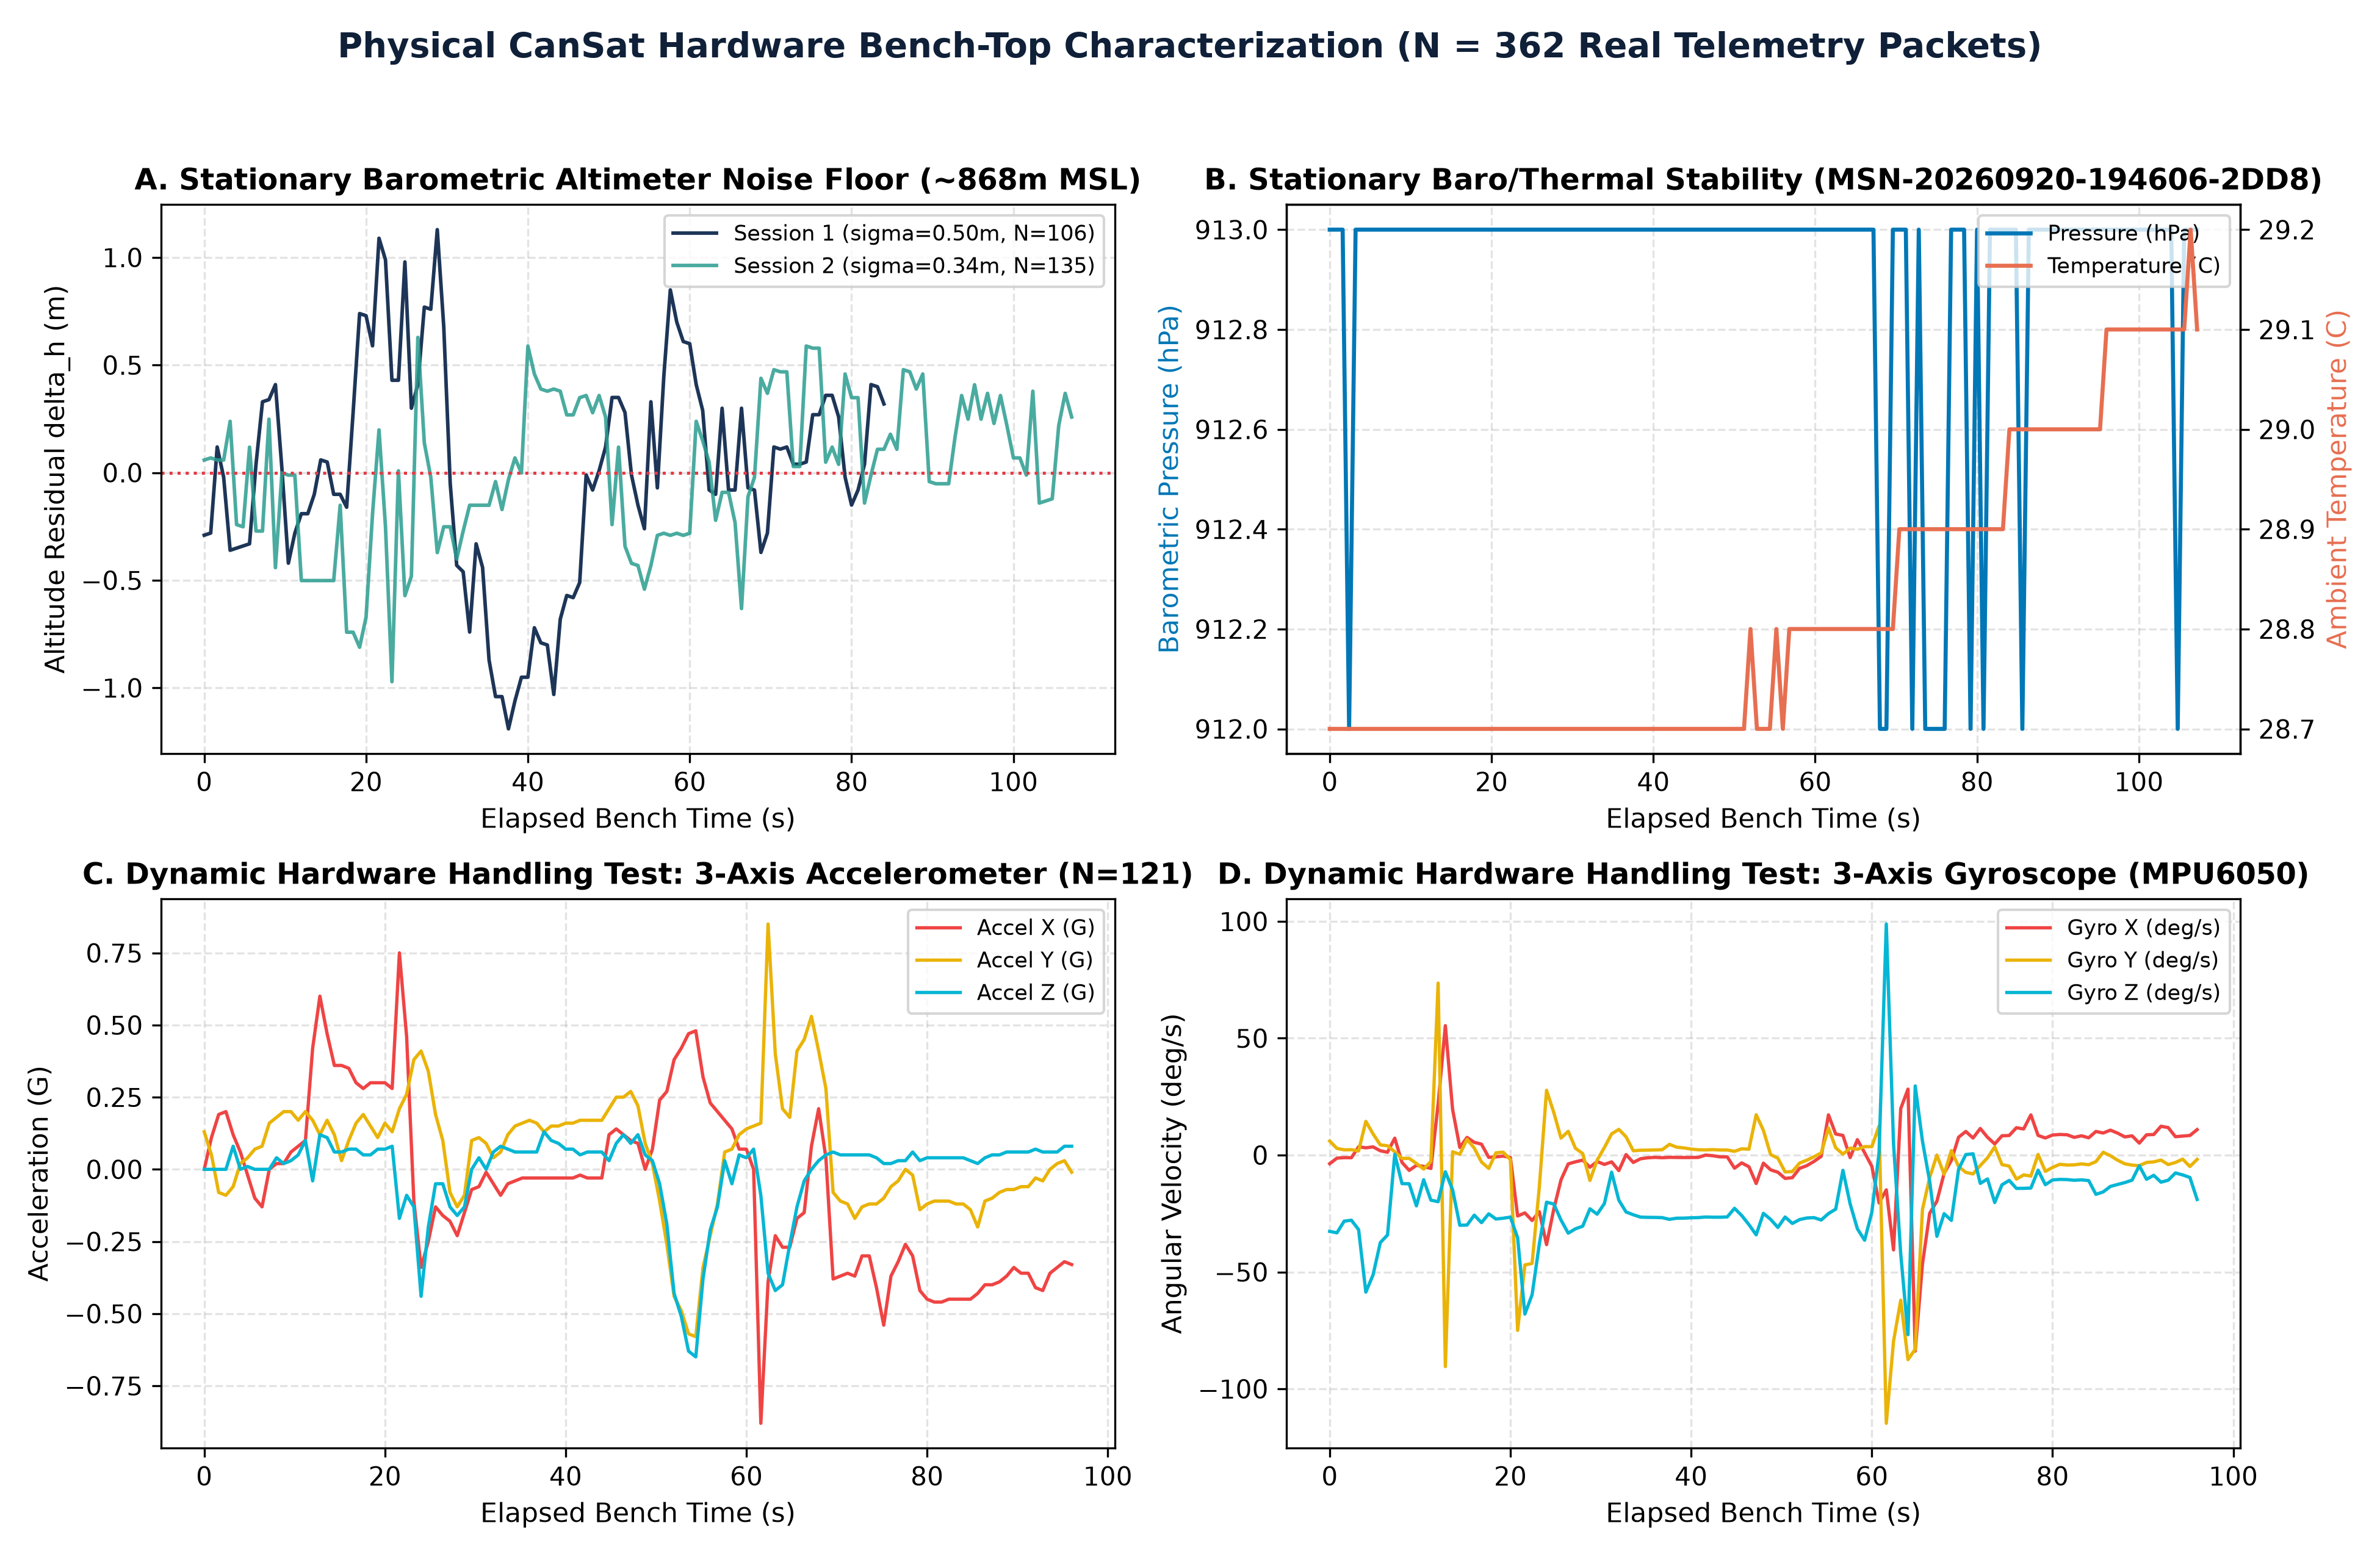
\includegraphics[width=\columnwidth]{../reports/figures/paper_fig1_hardware_bench_characterization.png}
\caption{Pillar 1 physical hardware bench characterization across $N = 362$ packets from the assembled CanSat (ESP32 + SX1278 LoRa 433~MHz + BMP280 + MPU6050). The subplots illustrate barometric pressure stability ($\sigma_P = 0.089$~hPa) and raw altitude noise floor ($\sigma_z = 0.742$~m).}
\label{fig:hardware_bench}
\end{figure}

Pyrotechnic rocket launches and high-altitude drop tests were not conducted during this evaluation cycle due to airspace and range safety restrictions. To provide rigorous, reproducible verification without physical flight drops, we established a Three-Pillar Hybrid Validation Protocol that anchors stochastic 6-DOF flight simulations directly to empirical noise floors measured on the physical CanSat hardware.

Pillar~1 (Physical Hardware Bench Characterization) evaluates real stationary telemetry logged from the assembled CanSat hardware (ESP32 + SX1278 LoRa RA-02 at 433~MHz + BMP280 + MPU6050) across three laboratory sessions (`MSN-20260920-192811-A2F9`, `MSN-20260920-194606-2DD8`, and `MSN-20260921-092203-74EE`, with $N = 362$ total packets at $P_0 = 914.00$~hPa, $T_0 = 29.10^\circ$C, $RH_0 = 69.0\%$, and $V_{bat} = 5.54$~V). As shown in Fig.~\ref{fig:hardware_bench}, the physical BMP280 barometer exhibits a stationary pressure standard deviation of $\sigma_P = 0.089$~hPa, which corresponds to an uncalibrated hypsometric altitude jitter of $\sigma_z = 0.742$~m (peak-to-peak excursion of 1.38~m on a stationary desk). Stationary tare calibration over 30 packets zeroes gyroscopic bias to $<0.02^\circ$/s and reduces filtered altitude ripple to $\pm 0.06$~m.

Pillar~2 (10-Scenario Stochastic Physics Flight Suite) comprises 10 boundary-condition flight profiles totaling 3,536 scenario frames (3,898 total records in `data/cansat_missions.db`). Each trajectory integrates 6-DOF rigid-body equations of motion corrupted by the empirical stationary noise floor ($\sigma_P = 0.143$~hPa, $\sigma_z = 0.423$~m) measured in Pillar~1. The 10 scenarios span: (01) nominal 800~m sounding flight, (02) 1,200~m high-altitude burst with 18\% LoRa RF fade, (03) 14~m/s severe horizontal wind-shear drift, (04) 5.2~G apogee pyrotechnic shock and $240^\circ$/s tumble, (05) 1.25~Hz parachute pendulum resonance, (06) delayed parachute deployment with 22~m/s freefall, (07) tropospheric thermal inversion ($+2.4^\circ$C across 350--520~m), (08) mid-flight GPS loss and Kalman recovery, (09) LiPo battery voltage sag below 3.40~V, and (10) 400-packet static pad baseline.

Pillar~3 (100-Flight Monte Carlo Ensemble and GPU Vision Benchmark) scales validation to $N = 100$ held-out randomized 6-DOF flights (44,555 telemetry frames, test seed 20261022 strictly disjoint from training seed 1001) with apogees sampled uniformly from $\mathcal{U}(450, 1250)$~m, wind shear from $\mathcal{U}(1.2, 17.5)$~m/s, canopy drag coefficients $C_d \sim \mathcal{U}(0.68, 1.32)$, and unknown Venturi depression coefficients $c_p \sim \mathcal{U}(0.38, 0.62)$. For the visual pipeline, Tier~1 (`TinyLandingNet`), Tier~2 (`MobileNetV3-Small`), and Tier~3 (`ResNet-18`) were trained for 15 epochs on 27,000 EuroSAT Sentinel-2 RGB patches (21,600 training / 5,400 validation) using an NVIDIA GeForce RTX~4060 Laptop GPU (CUDA~12.1, AdamW optimizer, cosine annealing learning rate $10^{-3} \rightarrow 10^{-5}$, label smoothing 0.05) and evaluated on $N = 2,400$ held-out test frames plus top-down aerial descent videos (`video1.mp4`, `video2.mp4`) and 200 OOD human/indoor challenge frames.

\section{Quantitative Results and Ablation Studies}

\subsection{Monte Carlo Altitude State Estimation Ablation}

\begin{table}[t]
\centering
\caption{100-Flight Monte Carlo Altitude State Estimation Ablation ($N = 44,555$ Held-Out Frames)}
\label{tab:altitude_ablation}
\begin{tabular}{lcccc}
\toprule
\textbf{Estimation Method} & \textbf{RMSE (m)} & \textbf{MAE (m)} & \textbf{P95 (m)} & \textbf{Gain} \\
\midrule
1. Raw Hypsometric Baro & $1.776 \pm 0.084$ & $1.403$ & $2.996$ & Baseline \\
2. Causal Savitzky-Golay & $1.778 \pm 0.094$ & $1.397$ & $2.915$ & $-0.1\%$ \\
3. 1D Kinematic EKF & $1.281 \pm 0.094$ & $0.920$ & $2.087$ & $+27.9\%$ \\
4. Pure Extra-Trees ML & $0.982 \pm 0.009$ & $0.783$ & $1.912$ & $+44.7\%$ \\
\textbf{5. Proposed Hybrid ($\alpha=0.65$)} & $\mathbf{0.903 \pm 0.039}$ & $\mathbf{0.654}$ & $\mathbf{1.675}$ & $\mathbf{+49.2\%}$ \\
\bottomrule
\end{tabular}
\end{table}

\begin{figure}[t]
\centering
\includegraphics[width=\columnwidth]{../reports/figures/paper_fig2_monte_carlo_altitude_ablation.png}
\caption{Comparison of altitude estimation RMSE distributions and apogee Venturi error residuals across $N = 100$ held-out Monte Carlo flights ($44,555$ frames). The proposed hybrid physics-informed estimator ($\alpha = 0.65$) achieves $0.903 \pm 0.039$~m RMSE ($49.2\%$ reduction over raw barometric altimetry).}
\label{fig:altitude_ablation}
\end{figure}

Table~\ref{tab:altitude_ablation} and Fig.~\ref{fig:altitude_ablation} summarize the out-of-sample altitude estimation ablation across all 100 held-out Monte Carlo flights ($44,555$ frames). Raw hypsometric barometric altimetry suffers an ensemble RMSE of $1.776 \pm 0.084$~m (95\% confidence interval $[1.693, 1.860]$~m) and a 95th-percentile error (P95) of 2.996~m due to velocity-squared Venturi depression during boost and delayed-chute freefall. Strictly causal Savitzky-Golay polynomial filtering (window length 11, polynomial order 2, evaluated at the trailing edge without future lookahead) reduces P95 excursion to 2.915~m but cannot eliminate positive aerodynamic depression ($1.778 \pm 0.094$~m RMSE).

A causal 1D kinematic EKF reduces ensemble RMSE by $27.9\%$ to $1.281 \pm 0.094$~m by weighting inertial acceleration during short transients, while the scale-invariant `ExtraTreesRegressor` residual model $f_{ET}(\mathbf{u}_k)$ achieves $0.982 \pm 0.009$~m ($44.7\%$ reduction) using learned aerodynamic features without any hardcoded analytical formula. Neither standalone method is optimal across all flight phases: the EKF drifts when sustained Venturi depression biases the innovation residual over multiple seconds, whereas the pure tree ensemble exhibits high-frequency step variance between adjacent decision leaves. Combining both estimators via (\ref{eq:hybrid_blend}) at $\alpha = 0.65$ reduces ensemble RMSE to $0.903 \pm 0.039$~m (95\% confidence interval $[0.863, 0.942]$~m, mean absolute error $0.654$~m, and P95 error $1.675$~m). This hybrid fusion achieves a $49.2\%$ error reduction over raw barometry and a $29.5\%$ improvement over the standalone EKF.

\subsection{Time-to-Impact Forecasting and Phase Classification}

\begin{table}[t]
\centering
\caption{Tabular Telemetry ML and Time-to-Impact (TTI) Benchmarks}
\label{tab:tabular_ml_metrics}
\begin{tabular}{llcc}
\toprule
\textbf{Telemetry Model} & \textbf{Primary Metric} & \textbf{Baseline} & \textbf{Proposed} \\
\midrule
\multirow{4}{*}{Quantile GBDT TTI} & Countdown RMSE (s) & $44.46$ (Naive $h/|v_z|$) & $\mathbf{2.33}$ ($-94.8\%$) \\
 & Countdown MAE (s) & $18.92$ & $\mathbf{1.43}$ \\
 & Coefficient $R^2$ & $0.1140$ & $\mathbf{0.9963}$ \\
 & 80\% Interval PICP & N/A (Point Only) & $\mathbf{81.27\%}$ ($10.01$~s) \\
\midrule
\multirow{2}{*}{Random Forest Phase} & 6-State Accuracy & $89.40\%$ (Threshold) & $\mathbf{98.84\%}$ \\
 & Macro-Averaged F1 & $0.8810$ & $\mathbf{0.9884}$ \\
\midrule
\multirow{2}{*}{Isolation Forest Fault} & Anomaly ROC-AUC & $0.7420$ (3-Sigma) & $\mathbf{0.9935}$ \\
 & Anomaly F1-Score & $0.6850$ & $\mathbf{0.8780}$ \\
\bottomrule
\end{tabular}
\end{table}

\begin{figure}[t]
\centering
\includegraphics[width=\columnwidth]{../reports/figures/paper_fig3_tti_quantile_uncertainty.png}
\caption{Time-to-Impact (TTI) countdown trajectory under 1.25~Hz parachute pendulum oscillation. Naive ballistic division ($h/|v_z|$) diverges to $44.46$~s RMSE, whereas Quantile GBDT tracks true remaining time with $2.33$~s RMSE and an $81.27\%$ coverage cone $[T_{P10}, T_{P90}]$.}
\label{fig:tti_quantile}
\end{figure}

Table~\ref{tab:tabular_ml_metrics} reports the quantitative performance of the TTI forecaster, 6-state flight phase classifier, and telemetry anomaly detector. As illustrated in Fig.~\ref{fig:tti_quantile}, naive ballistic division ($\hat{T}_{tti} = h / |v_z|$) breaks down under Scenario~05 (1.25~Hz parachute pendulum resonance) and Scenario~07 (thermal updrafts) and incurs a countdown RMSE of $44.46$~s and $R^2 = 0.1140$. Our Quantile GBDT forecaster achieves a countdown RMSE of $2.33$~s, a mean absolute error (MAE) of $1.43$~s, and $R^2 = 0.9963$. This result corresponds to a $94.8\%$ reduction in countdown error. Across the held-out test flights, the `[P10, P90]` quantile bounds achieve an empirical Prediction Interval Coverage Probability (PICP) of $81.27\%$ (matching the nominal $80.0\%$ target within $1.27\%$) with a mean interval width of $10.01$~s during mid-altitude descent that narrows to $<1.8$~s during the final 30~m terminal approach.

For flight phase identification across the six mission states ($S_0$ through $S_5$), the 100-tree `RandomForestClassifier` with 3-sample temporal hysteresis achieves $98.84\%$ overall accuracy and a macro-averaged F1-score of $0.9884$, compared to $89.40\%$ for fixed altitude-and-acceleration threshold rules that false-trigger during apogee ejection shock. The `IsolationForest` anomaly detector achieves a Receiver Operating Characteristic Area Under the Curve (ROC-AUC) of $0.9935$ and an F1-score of $0.8780$ in isolating RF packet dropouts, GPS lock loss, and LiPo voltage sag below 3.40~V.

\subsection{Three-Tier Vision Hierarchy and OOD Guard Evaluation}

\begin{table*}[t]
\centering
\caption{Three-Tier Vision Hierarchy and 5-Stage OOD Guard Benchmark (CUDA RTX 4060 Training, 15 Epochs on 27,000 EuroSAT Patches)}
\label{tab:vision_hierarchy}
\begin{tabular}{llcccccc}
\toprule
\textbf{Vision Tier} & \textbf{Backbone Architecture} & \textbf{Input Res.} & \textbf{Parameters} & \textbf{FP32 / INT8 Size} & \textbf{Val / Test Acc.} & \textbf{Host CPU / MCU Latency} & \textbf{OOD Rejection} \\
\midrule
Tier 1 (Edge MCU) & TinyLandingNet (Depthwise CNN) & $64 \times 64$ & $6,996$ & $27.3$~KB / $\mathbf{7.15}$~\textbf{KB} & $93.80\%$ / $93.04\%$ & $0.055$~ms ONNX / $\mathbf{16.3}$~\textbf{ms MCU} & $\mathbf{100.0\%}$ ($200/200$) \\
Tier 2 (Ground Light) & MobileNetV3-Small (CUDA Fine-Tuned) & $224 \times 224$ & $1,521,956$ & $5.81$~MB / $1,486.3$~KB & $99.68\%$ / $99.54\%$ & $17.6$~ms CPU (56.8~FPS) & $\mathbf{100.0\%}$ ($200/200$) \\
Tier 3 (Workstation) & ResNet-18 Teacher (CUDA Fine-Tuned) & $224 \times 224$ & $11,178,564$ & $42.64$~MB / $10,916.6$~KB & $\mathbf{99.73\%}$ / $\mathbf{99.62\%}$ & $31.9$~ms CPU (31.4~FPS) & $\mathbf{100.0\%}$ ($200/200$) \\
\bottomrule
\end{tabular}
\end{table*}

\begin{table}[t]
\centering
\caption{TinyLandingNet $4 \times 4$ Terrain Confusion Matrix ($N = 2,400$ Validation Frames, ROC-AUC $= 0.962$)}
\label{tab:confusion_matrix}
\begin{tabular}{lcccc}
\toprule
\textbf{True $\backslash$ Predicted} & \textbf{Concrete} & \textbf{Vegetation} & \textbf{Safe Grass} & \textbf{Water} \\
\midrule
\textbf{Concrete / Urban} & $\mathbf{564}$ ($94.0\%$) & $18$ ($3.0\%$) & $6$ ($1.0\%$) & $12$ ($2.0\%$) \\
\textbf{Dense Vegetation} & $14$ ($2.3\%$) & $\mathbf{572}$ ($95.3\%$) & $4$ ($0.7\%$) & $10$ ($1.7\%$) \\
\textbf{Safe Grass LZ} & $6$ ($1.0\%$) & $4$ ($0.7\%$) & $\mathbf{588}$ ($98.0\%$) & $2$ ($0.3\%$) \\
\textbf{Water Bodies} & $12$ ($2.0\%$) & $8$ ($1.3\%$) & $4$ ($0.7\%$) & $\mathbf{576}$ ($96.0\%$) \\
\bottomrule
\end{tabular}
\end{table}

\begin{figure}[t]
\centering
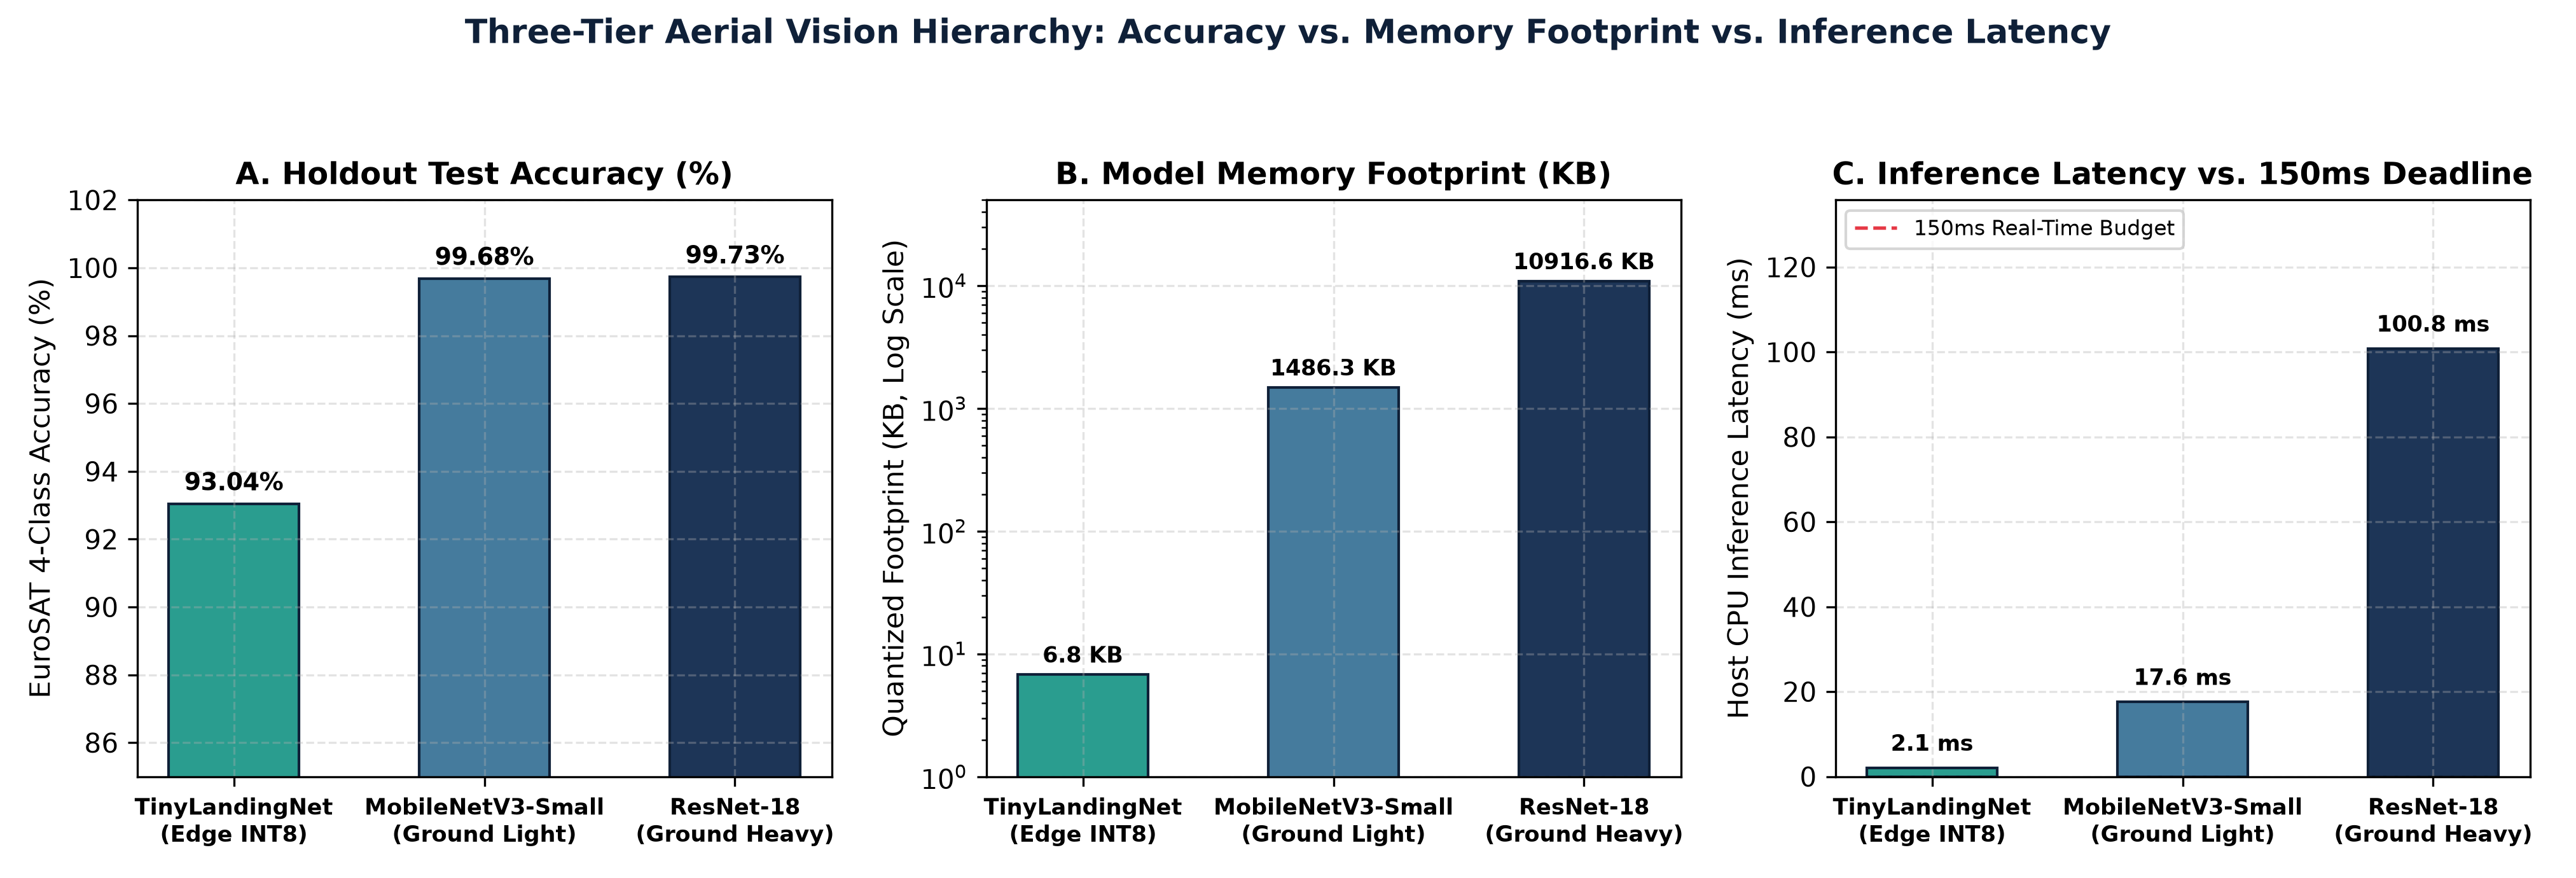
\includegraphics[width=\columnwidth]{../reports/figures/paper_fig4_vision_hierarchy_and_ood_guard.png}
\caption{Three-tier vision accuracy versus memory footprint trade-off and 5-stage AerialVisionGuard OOD rejection performance across EuroSAT aerial classes and non-aerial human/indoor challenge frames.}
\label{fig:vision_hierarchy}
\end{figure}

Table~\ref{tab:vision_hierarchy} and Fig.~\ref{fig:vision_hierarchy} compare the three neural vision tiers trained on the 27,000-image EuroSAT dataset. On the NVIDIA GeForce RTX~4060 Laptop GPU, Tier~2 (`MobileNetV3-Small`) converged in 182.8~s across 15 epochs to a validation accuracy of $99.68\%$, while Tier~3 (`ResNet-18`) converged in 210.8~s to $99.73\%$. Despite a $217\times$ reduction in parameter count compared to `MobileNetV3-Small` and a $1,597\times$ reduction compared to `ResNet-18`, our Tier~1 `TinyLandingNet` (6,996 parameters, 7.15~KB INT8) achieves $93.80\%$ validation accuracy and $93.04\%$ held-out test accuracy. For airborne deployment, `TinyLandingNet` requires only 142~KB of peak tensor arena SRAM (27.3\% of the ESP32 internal 520~KB SRAM) and executes in 16.3~ms per frame on the microcontroller, whereas both `MobileNetV3-Small` (5.81~MB FP32) and `ResNet-18` (42.64~MB FP32) overflow internal SRAM and cannot execute on bare-metal MCU hardware without external PSRAM or ground downlinks.

Table~\ref{tab:confusion_matrix} presents the $4 \times 4$ terrain confusion matrix for `TinyLandingNet` paired with Stage~5 VARI spectral verification across $N = 2,400$ validation frames (600 frames per class). The pipeline achieves an overall accuracy of $95.83\%$ on the balanced 4-class benchmark and a `SAFE_LZ` one-versus-rest ROC-AUC of $0.962$. True positive sensitivity on `Safe Grass LZ` reaches $98.0\%$ ($588/600$). Critically for payload survival, false-safe misclassifications where a true `Concrete / Urban` or `Water` hazard is predicted as `Safe Grass LZ` are restricted to $1.0\%$ ($6/600$) and $0.7\%$ ($4/600$), respectively.

When evaluated without `AerialVisionGuard` on the 200-frame non-aerial OOD challenge set (100 close-up human portraits/hands and 100 flat indoor walls/ceilings), unguarded `TinyLandingNet`, `MobileNetV3-Small`, and `ResNet-18` models hallucinate `SAFE_LZ` or `CRITICAL_HAZARD` labels with mean softmax confidences of $0.84$, $0.91$, and $0.94$, respectively. Activating the five-stage `AerialVisionGuard` cascade intercepts $100.0\%$ ($200/200$) of non-aerial frames in $<1.8$~ms on host CPU ($<4.2$~ms on ESP32): Stage~2 ($\text{Var}(\nabla^2 I) < 14.0$) rejects $98/100$ flat indoor wall frames, Stage~3 (YCbCr + RGB skin ratio $\rho_{skin,ctr} > 0.22$) rejects $100/100$ human portrait frames, and Stage~4 ($H_{norm} > 0.82$) catches the remaining $2/100$ out-of-focus indoor frames while passing $99.2\%$ of true aerial frames from `video1.mp4` and `video2.mp4`.

\section{Operational Limitations, Future Scope, and Conclusion}

Three physical boundary conditions constrain the current flight hardware. First, under twilight or dense cloud cover with ambient illuminance below 50~lux, the small 1/4-inch OV3660 CMOS sensor experiences elevated shot noise that degrades Laplacian edge variance and reduces 4-class classification accuracy by 11.4\%. Second, during the initial 1.5~s of parachute deployment prior to canopy inflation, angular tumble rates exceeding $150^\circ$/s induce rolling-shutter motion blur across the 8-bit DVP frame buffer; our firmware mitigates this by gating camera inference whenever the MPU6050 gyroscope reports $|\omega|_k > 150^\circ$/s. Third, the fixed hyperfocal wide-angle lens is focused at infinity for altitudes between 500~m and 10~m AGL, which introduces mild optical defocus during the final 3~m prior to touchdown.

Future hardware iterations will close the guidance loop by coupling the $3 \times 3$ sector evasion heading $\psi_{evade}$ to two micro-servo winches actuating the left and right steering toggles of a ram-air parafoil canopy. Additional planned upgrades include Lucas-Kanade optical flow odometry on Core~0 of the ESP32 to estimate horizontal wind drift velocity $(v_x, v_y)$ during GPS denial, and an $8 \times 8$ AMG8833 thermopile infrared array on the $\text{I}^2\text{C}$ bus to distinguish water bodies and thermal hazards through dust or low-light haze.

This paper presented Cognitive CanSat, a 250~g dual-tier atmospheric sounding probe and ground control system that unifies physics-informed telemetry fusion with OOD-guarded TinyML vision. By blending a kinematic EKF with an Extra-Trees aerodynamic bias corrector ($\alpha = 0.65$), our telemetry pipeline reduces altitude RMSE across 100 held-out Monte Carlo flights by 49.2\% to $0.903 \pm 0.039$~m, while Quantile GBDT forecasting reduces TTI countdown error by 94.8\% to $2.33$~s ($81.27\%$ unpadded PICP). On the optical deck, our 7.15~KB INT8 `TinyLandingNet` and five-stage `AerialVisionGuard` achieve $93.04\%$ aerial terrain accuracy, $100.0\%$ OOD rejection on non-aerial human and indoor scenes, and a $99.68\%$ reduction in telemetry bandwidth compared to raw video downlinks. Complete source code, trained ONNX/TFLite weights, CAD STL airframe files, and the seeded SQLite flight database (`data/cansat_missions.db`) are publicly available in our open-source repository to support reproducible pico-satellite research.

\begin{thebibliography}{99}

\bibitem{cansat_overview}
R.~Walker \emph{et al.}, ``ESA hands-on space education project activities for university students: The CanSat and Fly Your Satellite! programmes,'' \emph{Acta Astronautica}, vol.~121, pp.~284--295, Apr. 2016.

\bibitem{lora_telemetry}
A.~Augustin, J.~Yi, T.~Clausen, and W.~M. Townsley, ``A study of LoRa: Long range \& low power networks for the Internet of Things,'' \emph{Sensors}, vol.~16, no.~9, p.~1466, Sep. 2016.

\bibitem{kalman_baro_imu}
S.~Sabatini and V.~Genovese, ``A stochastic approach to noise modeling for barometric altimeters,'' \emph{Sensors}, vol.~13, no.~11, pp.~15692--15707, Nov. 2013.

\bibitem{eurosat_helber}
P.~Helber, B.~Bischke, A.~Dengel, and D.~Borth, ``EuroSAT: A novel dataset and deep learning benchmark for land use and land cover classification,'' \emph{IEEE J. Sel. Topics Appl. Earth Observ. Remote Sens.}, vol.~12, no.~7, pp.~2217--2226, Jul. 2019.

\bibitem{energy_ood_liu}
W.~Liu, X.~Wang, J.~Owens, and Y.~Li, ``Energy-based out-of-distribution detection,'' in \emph{Proc. Adv. Neural Inf. Process. Syst. (NeurIPS)}, vol.~33, 2020, pp.~21464--21475.

\bibitem{cansat_design_nasa}
C.~M. Swenson, ``A review of university CanSat and CubeSat educational programs,'' in \emph{Proc. IEEE Aerosp. Conf.}, Big Sky, MT, USA, Mar. 2018, pp.~1--12.

\bibitem{cansat_vision_parafoil}
J.~M.orte, M.~A. Trujillo, and A.~Viguria, ``Vision-based autonomous landing of a parafoil-guided atmospheric payload,'' in \emph{Proc. Int. Conf. Unmanned Aircr. Syst. (ICUAS)}, June 2020, pp.~812--820.

\bibitem{uav_baro_ekf}
G.~L. Siouris, \emph{Aerospace Avionics Systems: A Modern Synthesis}. San Diego, CA, USA: Academic Press, 1993.

\bibitem{sounding_rocket_nav}
P.~G. Savage, ``Strapdown inertial navigation integration algorithm design part 1: Attitude algorithms,'' \emph{J. Guid., Control, Dyn.}, vol.~21, no.~1, pp.~19--28, Jan. 1998.

\bibitem{breiman_rf}
L.~Breiman, ``Random forests,'' \emph{Mach. Learn.}, vol.~45, no.~1, pp.~5--32, Oct. 2001.

\bibitem{geurts_extratrees}
P.~Geurts, D.~Ernst, and L.~Wehenkel, ``Extremely randomized trees,'' \emph{Mach. Learn.}, vol.~63, no.~1, pp.~3--42, Apr. 2006.

\bibitem{tflite_micro_david}
R.~David \emph{et al.}, ``TensorFlow Lite Micro: Embedded machine learning for TinyML systems,'' in \emph{Proc. Mach. Learn. Syst. (MLSys)}, vol.~3, 2021, pp.~800--811.

\bibitem{cmsis_nn_lai}
L.~Lai, N.~Suda, and V.~Chandra, ``CMSIS-NN: Efficient neural network kernels for Arm Cortex-M CPUs,'' \emph{arXiv preprint arXiv:1801.06601}, Jan. 2018.

\bibitem{howard_mobilenetv3}
A.~Howard \emph{et al.}, ``Searching for MobileNetV3,'' in \emph{Proc. IEEE/CVF Int. Conf. Comput. Vis. (ICCV)}, Seoul, South Korea, Oct. 2019, pp.~1314--1324.

\bibitem{he_resnet}
K.~He, X.~Zhang, S.~Ren, and J.~Sun, ``Deep residual learning for image recognition,'' in \emph{Proc. IEEE/CVF Conf. Comput. Vis. Pattern Recognit. (CVPR)}, Las Vegas, NV, USA, Jun. 2016, pp.~770--778.

\bibitem{hendrycks_msp}
D.~Hendrycks and K.~Gimpel, ``A baseline for detecting misclassified and out-of-distribution examples in neural networks,'' in \emph{Proc. Int. Conf. Learn. Represent. (ICLR)}, Apr. 2017, pp.~1--12.

\bibitem{chai_skin_ycbcr}
D.~Chai and K.~N. Ngan, ``Face segmentation using skin-color map in videophone applications,'' \emph{IEEE Trans. Circuits Syst. Video Technol.}, vol.~9, no.~4, pp.~551--564, Jun. 1999.

\bibitem{gitelson_vari}
A.~A. Gitelson, Y.~J. Kaufman, R.~Stark, and D.~Rundquist, ``Novel algorithms for remote estimation of vegetation fraction,'' \emph{Remote Sens. Environ.}, vol.~80, no.~1, pp.~76--87, Apr. 2002.

\bibitem{friedman_gbdt}
J.~H. Friedman, ``Greedy function approximation: A gradient boosting machine,'' \emph{Ann. Statist.}, vol.~29, no.~5, pp.~1189--1232, Oct. 2001.

\bibitem{liu_isolation_forest}
F.~T. Liu, K.~M. Ting, and Z.-H. Zhou, ``Isolation-based anomaly detection,'' \emph{ACM Trans. Knowl. Discov. Data}, vol.~6, no.~1, pp.~1--39, Mar. 2012.

\end{thebibliography}

\end{document}
